\documentclass[a4,10pt,comentarios]{aleph-notas}
\usepackage{aleph-comandos}
\usepackage{enumitem}
\usepackage{amssymb}
\usepackage{hyperref}
\usepackage{multicol}
\usepackage{amsmath}
\usepackage{graphicx}
\usepackage{listings}
\usepackage{algorithm}
\usepackage[parfill]{parskip}
\usepackage[noend]{algpseudocode}
\fuente{montserrat}
\graphicspath{ {./img/} }
\setlength{\headheight}{44pt}

% -- Datos de la tarea
\institucion{Criptografía y Seguridad}
\autor{Uziel Vidal Cruz Vargas\\
Emilio Arsenio Raudry Rico}
\tema{Práctica 02: Explotación de vulnerabilidades:\\
desbordamiento de búfer.}

\logouno[9cm]{img/fc}
\begin{document}

\encabezado

\section{Recopilación}

Cada uno de los dos programas cuenta con una función la cual solo es accesible si ingresamos una contraseña correcta. Nuestra prueba consiste en probar lo opuesto, demostrar que podemos acceder a dichas funciones (y la información que estas contienen) sin necesidad de si quiera usar las contraseñas.

Al tratarse de una prueba de caja blanca, contamos ya con el código fuente, el cual nos servirá para que sepamos qué direcciones de memoria acceder más adelante. Para el punto anterior nos apoyaremos en la herramienta GDB.

Como nuestro ataque será mediante un buffer overflow, también necesitaremos una herramienta con estructuras de flujo iterativas como python3.

Finalmente, como tratamos con un tipo de ataque altamente conocido y tratado a lo largo de los años, partiremos de que la aleatoriedad de espacio de direcciones virtuales en el kernel de Linux se encuentra desactivado. Esto lo podemos lograr con el comando:

\begin{center}
    \texttt{sudo sysctl -w kernel.randomize\_va\_space=0}
\end{center}
\section{Explotación}

Dado que ambos códigos hacen uso de una función considerada peligrosa, por lo que para poder compilarlo tendremos que proveerle a \textit{gcc} ciertas banderas:

\begin{quote}
\texttt{gcc -g -fno-stack-protector -z execstack nombreCodigo.c -o nombreCodigoCompilado -std=c99 -D\_FORTIFY\_SOURCE=0}
\end{quote}

\begin{center}
    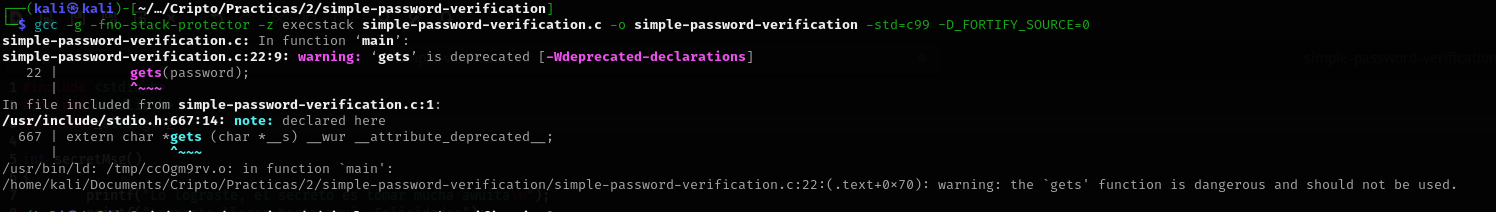
\includegraphics[scale=.3]{img/compilePassword.png}
\end{center}

\begin{center}
    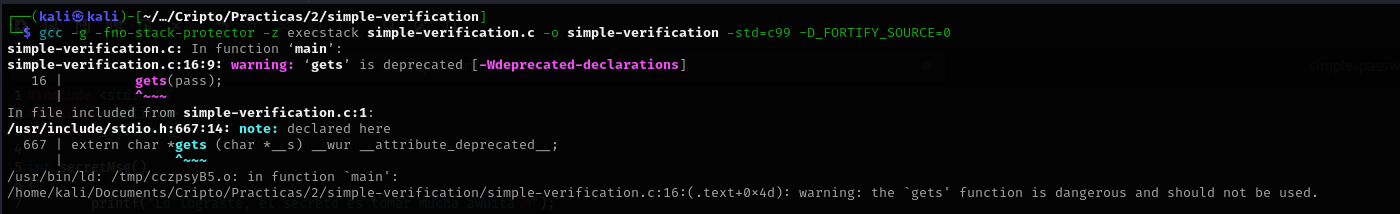
\includegraphics[scale=.3]{img/compileVerification.png}
\end{center}

Estas nos permiten indicarle al compilador lo siguiente:

\begin{itemize}
  \item \texttt{-g} Hace que el compilador incluya información de depuración que necesitaremos cuando usemos a GDB.
  \item \texttt{-fno-stack-protector} Hace que se desactive la protección del stack.
  \item \texttt{-z execstack} Hace que se pueda ejecutar código en el stack.
  \item \texttt{-std=c99} Establece el estándar C99.
  \item \texttt{-D\_FORTIFY\_SOURCE=0} Desactiva las optimizaciones de seguridad en las funciones de manejo de cadenas y buffers.
\end{itemize}

Una vez compilado el programa podemos ejecutarlo con GDB.

Lo ejecutamos de forma depurada con el comando \texttt{start}.

En el primer código, deseamos acceder a la función \texttt{granted()}, por lo que debemos de buscar su ubicación dentro del stack. Para ello podemos usar el siguiente comando de GDB \texttt{print granted}:

Hacemos lo mismo para el segundo código, donde el nombre de la función que buscamos es \texttt{secretMsg()}, ejecutando así en GDB \texttt{print secretMsg}:

\begin{center}
    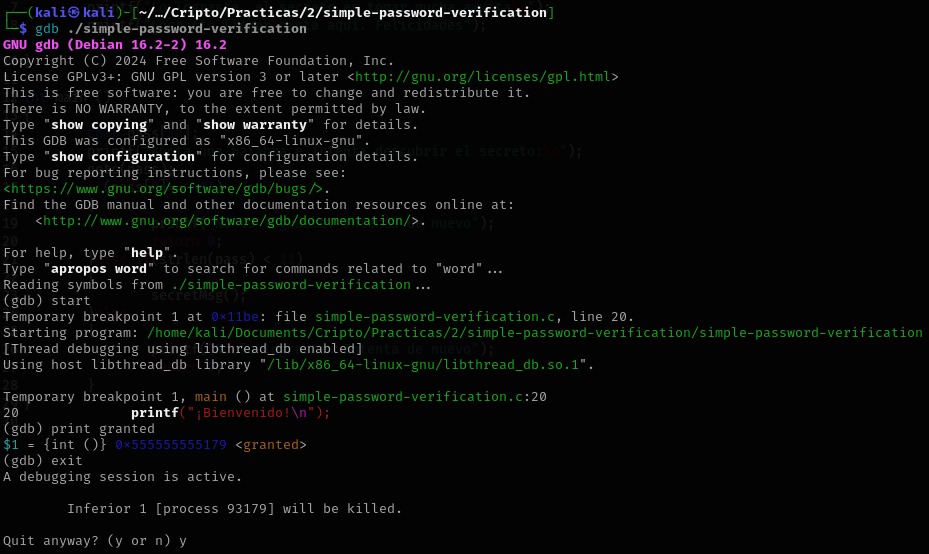
\includegraphics[scale=.5]{img/gdbPassword.png}
\end{center}

\begin{center}
    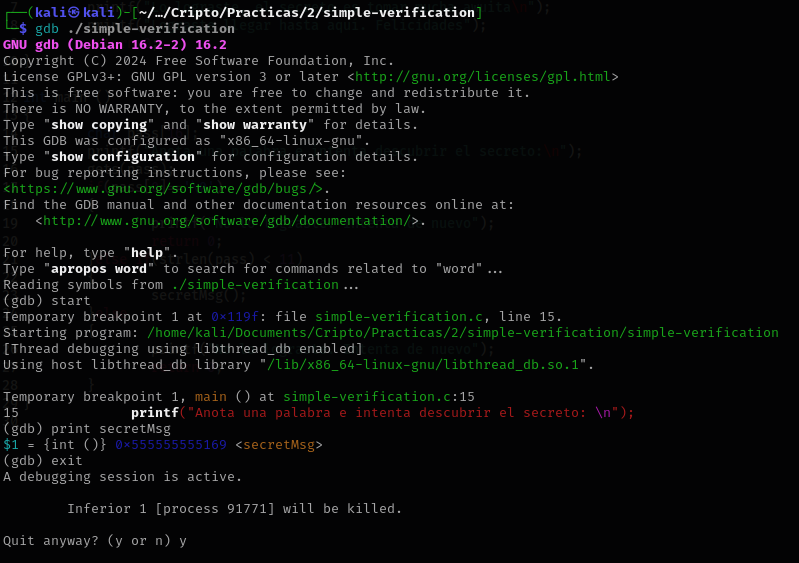
\includegraphics[scale=.5]{img/gdbVerification.png}
\end{center}

Anotamos las direcciones de ambas y salimos de GDB. El motivo de esto, es que, una vez que llenemos el buffer con su máxima capacidad, podamos escribir en el registro de dirección de retorno del stack, la dirección de memoria de dichas funciones.

De esta manera, nuestro exploit consistirá en una entrada de tipo string compuesta por una cantidad caracteres igual al límite del buffer concatenados con la dirección de memoria de ambas funciones. 

Una observación importante es que al momento de que la computadora lea la dirección de memoria, esta debe de estar en formato little endian, la cual consiste en dividir la dirección original en parejas de caracteres y añadirlos en una cadena en orden inverso, donde cada pareja le preceden los caracteres \texttt{\textbackslash x}.

Para realizar estos nos apoyaremos de python, de manera que nuestro exploit se ejecute bajo el siguiente comando:

\begin{quote}
\texttt{python3 -c 'print(''A''*\{límite del buffer\} + "[dirección de memoria de la función]") | ./[nombre del programa compilado]'}
\end{quote}


La bandera \texttt{-c} permite ejecutar python3 desde la línea de comandos. Hacemos que imprima una cantidad de caracteres igual al límite del buffer (en este caso usaremos a la letra A), y le concatenamos la dirección de la función en little endian. Dicha salida se la pasamos a nuestro programa para que la reciba como entrada al momento de ejecutarse.

Al momento de probar el exploit, intentamos con 16 A's (pues el es el tamaño de los dos arreglos que contienen nuestra entrada en los códigos), al no bastar les incrementamos uno hasta llegar al número 24.

De manera que para el primer código, el exploit quedó de la siguiente manera:

\begin{quote}
\texttt{python3 -c 'print(''A''*24 + "\textbackslash x79\textbackslash x51\textbackslash x55\textbackslash x55\textbackslash x55\textbackslash x55") | ./simple-password-verification'}
\end{quote}

\begin{center}
    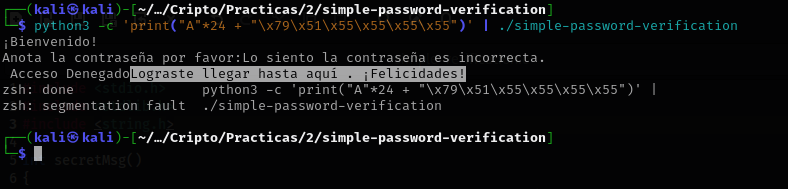
\includegraphics[scale=.5]{img/exploitPassword.png}
\end{center}

Mientras que para el segundo código, quedó así:

\begin{quote}
\texttt{python3 -c 'print(''A''*24 + "\textbackslash x69\textbackslash x51\textbackslash x55\textbackslash x55\textbackslash x55\textbackslash x55") | ./simple-verification'}
\end{quote}

\begin{center}
    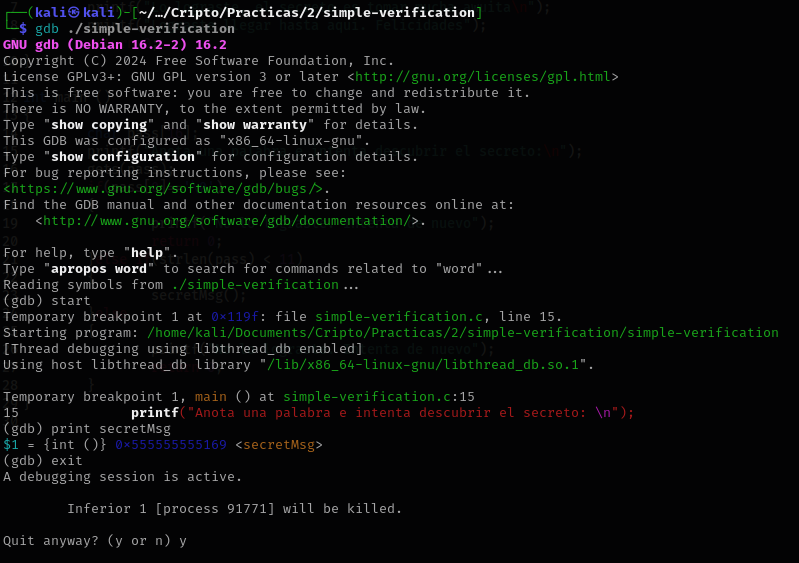
\includegraphics[scale=.5]{img/gdbVerification.png}
\end{center}

Podemos ver que en ambos casos, se pudo acceder a la función adecuada, pues recibimos los mensajes de aceptación.
\section{Post-explotación}

Lo que hicimos básicamente fue darle de entrada a los programas una cadena compuesta por dos partes. La primera subcadena consistió en una cantidad de letras \texttt{A} lo suficientemente grande para poder llenar el espacio designado en el stack al buffer. La segunda subcadena consistía en la dirección de la función a la que buscamos acceder.

El exploit es capaz de llevarnos a la ejecución de dicha función, pues dentro del stack, el bloque del buffer se encuentra justo al lado del bloque de la dirección de retorno. Esto hace que al momento de acceder a dicho bloque, en lugar de volver a la dirección de retorno de la llamada inicial, nos lleve a la que nosotros pusimos.

De esta manera, en ambos casos llegamos los bloque de código que queríamos sin tener que poner las contraseñas requeridas.

Para poder mejorar la seguridad del código, de entrada, no hay que usar funciones de bajo nivel tan inseguras como \texttt{gets()}. Siendo preferibles el uso de otras funciones para recibir entradas, como lo es \texttt{fgets()}. El cual comprueba el tamaño de la entrada para evitar desbordamientos.

No obstante, el mejoramiento no se debe limitar únicamente a eso. 

El primer código hace una llamada al sistema directamente, el cual, tras esta práctica acaba de demostrar lo peligroso que es esto, pues abre una ventana para poder modificar todo el sistema. (Es incluso por esta razón, el porqué no es recomendable darle a lenguajes de programación, la posibilidad de ser ejecutados como root por cualquier usuario).

Otra opción es la inclusión de control de errores, ya que, a pesar de tener métodos seguros, es mejor establecer una lógica robusta que ni siquiera le de la oportunidad al usuario de alcanzar casos críticos.

Otro añadido, que debería considerar más por convención que por otra cosa, es que al momento de hacer las verificaciones de las contraseñas, estas no se hagan en texto plano, si no bajo un hasheo. Esto tampoco es enteramente seguro, pues pude haber ataques de diccionario o fuerza bruta, pero impide una presencia explícita de la contraseña en el código.
\section{Alcance}
El alcance de un desbordamiento de buffer es igual de amplio que el alcance que pude tener la función a la que queramos acceder desde su dirección en el  \texttt{stack}.

En la función \texttt{granted()} (que accedimos en el primer código) hay una línea que abre la terminal de gnome (aunque por la configuración de nuestra máquina virtual, esta no se pudo abrir). Lo que nos puede permitir hacer modificaciones en el sistema e incluso, la posibilidad de escalar privilegios para poder hacer todo lo que queramos siendo root.

También puede ser que la función a la que llamemos, nos permita acceder información sensible, como lo fue con \texttt{secretMsg()}, que podamos robar, o incluso ocupar después para hacer movimientos laterales o causar mayores daños.


\bibliographystyle{plain}
\bibliography{referencias}

\end{document}